

\tikzset{every picture/.style={line width=0.75pt}} %set default line width to 0.75pt        

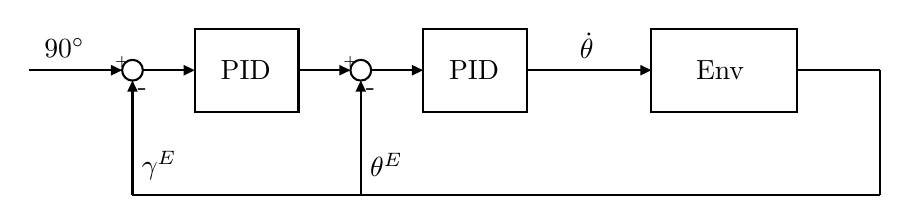
\begin{tikzpicture}[x=0.75pt,y=0.75pt,yscale=-1,xscale=1]
%uncomment if require: \path (0,300); %set diagram left start at 0, and has height of 300

%Shape: Rectangle [id:dp08340231298295664] 
\draw   (305,10) -- (375,10) -- (375,50) -- (305,50) -- cycle ;
%Shape: Rectangle [id:dp7804893715866246] 
\draw   (195,10) -- (245,10) -- (245,50) -- (195,50) -- cycle ;
%Shape: Rectangle [id:dp10510994638607651] 
\draw   (85,10) -- (135,10) -- (135,50) -- (85,50) -- cycle ;
%Straight Lines [id:da4873195092509457] 
\draw    (375,30) -- (415,30) ;
%Straight Lines [id:da5213289762000781] 
\draw    (415,30) -- (415,90) ;
%Straight Lines [id:da8653117319619519] 
\draw    (55,90) -- (415,90) ;
%Straight Lines [id:da20383266774784436] 
\draw    (245,30) -- (302,30) ;
\draw [shift={(305,30)}, rotate = 180] [fill={rgb, 255:red, 0; green, 0; blue, 0 }  ][line width=0.08]  [draw opacity=0] (5.36,-2.57) -- (0,0) -- (5.36,2.57) -- cycle    ;
%Shape: Circle [id:dp7361632364335162] 
\draw   (160,30) .. controls (160,27.24) and (162.24,25) .. (165,25) .. controls (167.76,25) and (170,27.24) .. (170,30) .. controls (170,32.76) and (167.76,35) .. (165,35) .. controls (162.24,35) and (160,32.76) .. (160,30) -- cycle ;
%Straight Lines [id:da7448530265787932] 
\draw    (165,90) -- (165,38) ;
\draw [shift={(165,35)}, rotate = 450] [fill={rgb, 255:red, 0; green, 0; blue, 0 }  ][line width=0.08]  [draw opacity=0] (5.36,-2.57) -- (0,0) -- (5.36,2.57) -- cycle    ;
%Straight Lines [id:da08688379307117211] 
\draw    (170,30) -- (192,30) ;
\draw [shift={(195,30)}, rotate = 180] [fill={rgb, 255:red, 0; green, 0; blue, 0 }  ][line width=0.08]  [draw opacity=0] (5.36,-2.57) -- (0,0) -- (5.36,2.57) -- cycle    ;
%Straight Lines [id:da8748724429291457] 
\draw    (135,30) -- (157,30) ;
\draw [shift={(160,30)}, rotate = 180] [fill={rgb, 255:red, 0; green, 0; blue, 0 }  ][line width=0.08]  [draw opacity=0] (5.36,-2.57) -- (0,0) -- (5.36,2.57) -- cycle    ;
%Shape: Circle [id:dp8312837604592662] 
\draw   (50,30) .. controls (50,27.24) and (52.24,25) .. (55,25) .. controls (57.76,25) and (60,27.24) .. (60,30) .. controls (60,32.76) and (57.76,35) .. (55,35) .. controls (52.24,35) and (50,32.76) .. (50,30) -- cycle ;
%Straight Lines [id:da6345780351972454] 
\draw    (55,90) -- (55,38) ;
\draw [shift={(55,35)}, rotate = 450] [fill={rgb, 255:red, 0; green, 0; blue, 0 }  ][line width=0.08]  [draw opacity=0] (5.36,-2.57) -- (0,0) -- (5.36,2.57) -- cycle    ;
%Straight Lines [id:da26670434464575177] 
\draw    (60,30) -- (82,30) ;
\draw [shift={(85,30)}, rotate = 180] [fill={rgb, 255:red, 0; green, 0; blue, 0 }  ][line width=0.08]  [draw opacity=0] (5.36,-2.57) -- (0,0) -- (5.36,2.57) -- cycle    ;
%Straight Lines [id:da5698237977531111] 
\draw    (5,30) -- (47,30) ;
\draw [shift={(50,30)}, rotate = 180] [fill={rgb, 255:red, 0; green, 0; blue, 0 }  ][line width=0.08]  [draw opacity=0] (5.36,-2.57) -- (0,0) -- (5.36,2.57) -- cycle    ;

% Text Node
\draw (325,24) node [anchor=north west][inner sep=0.75pt]   [align=left] {Env};
% Text Node
\draw (206,24) node [anchor=north west][inner sep=0.75pt]   [align=left] {PID};
% Text Node
\draw (96,24) node [anchor=north west][inner sep=0.75pt]   [align=left] {PID};
% Text Node
\draw (155,22) node [anchor=north west][inner sep=0.75pt]   [align=left] {{\tiny +}};
% Text Node
\draw (166,35) node [anchor=north west][inner sep=0.75pt]   [align=left] {\mbox{-}};
% Text Node
\draw (11,13.4) node [anchor=north west][inner sep=0.75pt]    {$90^{\circ }$};
% Text Node
\draw (58,67.4) node [anchor=north west][inner sep=0.75pt]    {$\gamma ^{E}$};
% Text Node
\draw (168,68.4) node [anchor=north west][inner sep=0.75pt]    {$\theta ^{E}$};
% Text Node
\draw (269,10.4) node [anchor=north west][inner sep=0.75pt]    {$\dot{\theta }$};
% Text Node
\draw (45,22) node [anchor=north west][inner sep=0.75pt]   [align=left] {{\tiny +}};
% Text Node
\draw (56,35) node [anchor=north west][inner sep=0.75pt]   [align=left] {\mbox{-}};


\end{tikzpicture}
